\begin{minipage}{0.75\linewidth}
\begin{figure}[h]
    \centering
    \begin{adjustbox}{max width=1.0\linewidth, keepaspectratio}
        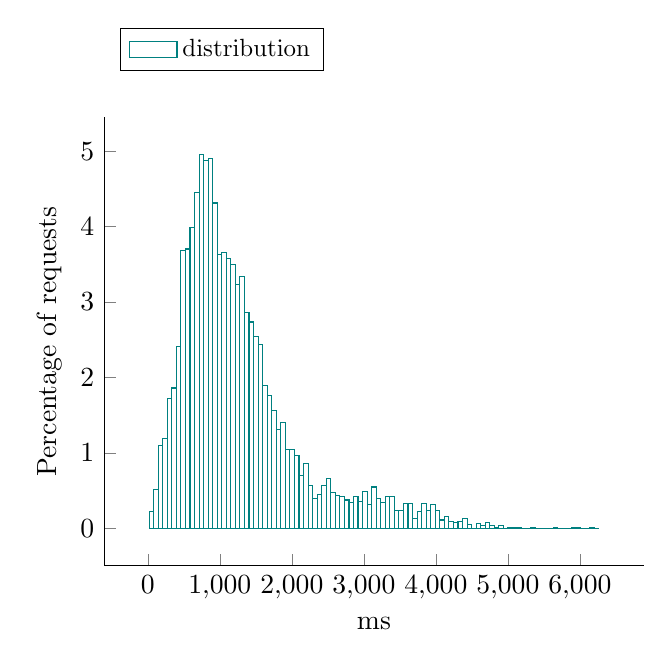
\begin{tikzpicture}
            \begin{axis}[ylabel = Percentage of requests, 
xlabel = ms, 
legend style = {nodes={scale=0.9, transform shape}, at={(0.03,1.2)}, anchor=north west, draw=black, fill=white, align=left, legend columns=3},
area style, mark size = 0pt,
 cycle list name = exotic,
  axis lines* = left]
		\addplot +[ybar interval] coordinates {
			 (18, 0.21875)
			 (81.07, 0.515625)
			 (144.14, 1.09375)
			 (207.21, 1.1875)
			 (270.28, 1.71875)
			 (333.35, 1.85938)
			 (396.42, 2.40625)
			 (459.49, 3.6875)
			 (522.56, 3.70312)
			 (585.63, 3.98437)
			 (648.7, 4.45312)
			 (711.77, 4.95312)
			 (774.84, 4.875)
			 (837.91, 4.90625)
			 (900.98, 4.3125)
			 (964.05, 3.625)
			 (1027.12, 3.65625)
			 (1090.19, 3.57812)
			 (1153.26, 3.5)
			 (1216.33, 3.23437)
			 (1279.4, 3.34375)
			 (1342.47, 2.85938)
			 (1405.54, 2.73438)
			 (1468.61, 2.54688)
			 (1531.68, 2.4375)
			 (1594.75, 1.89062)
			 (1657.82, 1.76562)
			 (1720.89, 1.5625)
			 (1783.96, 1.3125)
			 (1847.03, 1.40625)
			 (1910.1, 1.04688)
			 (1973.17, 1.04688)
			 (2036.24, 0.96875)
			 (2099.31, 0.703125)
			 (2162.38, 0.859375)
			 (2225.45, 0.5625)
			 (2288.52, 0.390625)
			 (2351.59, 0.453125)
			 (2414.66, 0.5625)
			 (2477.73, 0.65625)
			 (2540.8, 0.46875)
			 (2603.87, 0.4375)
			 (2666.94, 0.421875)
			 (2730.01, 0.375)
			 (2793.08, 0.34375)
			 (2856.15, 0.421875)
			 (2919.22, 0.359375)
			 (2982.29, 0.484375)
			 (3045.36, 0.3125)
			 (3108.43, 0.546875)
			 (3171.5, 0.390625)
			 (3234.57, 0.34375)
			 (3297.64, 0.421875)
			 (3360.71, 0.421875)
			 (3423.78, 0.234375)
			 (3486.85, 0.234375)
			 (3549.92, 0.328125)
			 (3612.99, 0.328125)
			 (3676.06, 0.125)
			 (3739.13, 0.21875)
			 (3802.2, 0.328125)
			 (3865.27, 0.234375)
			 (3928.34, 0.3125)
			 (3991.41, 0.234375)
			 (4054.48, 0.109375)
			 (4117.55, 0.15625)
			 (4180.62, 0.09375)
			 (4243.69, 0.078125)
			 (4306.76, 0.09375)
			 (4369.83, 0.125)
			 (4432.9, 0.046875)
			 (4495.97, 0)
			 (4559.04, 0.0625)
			 (4622.11, 0.03125)
			 (4685.18, 0.078125)
			 (4748.25, 0.03125)
			 (4811.32, 0.015625)
			 (4874.39, 0.03125)
			 (4937.46, 0)
			 (5000.53, 0.015625)
			 (5063.6, 0.015625)
			 (5126.67, 0.015625)
			 (5189.74, 0)
			 (5252.81, 0)
			 (5315.88, 0.015625)
			 (5378.95, 0)
			 (5442.02, 0)
			 (5505.09, 0)
			 (5568.16, 0)
			 (5631.23, 0.015625)
			 (5694.3, 0)
			 (5757.37, 0)
			 (5820.44, 0)
			 (5883.51, 0.015625)
			 (5946.58, 0.015625)
			 (6009.65, 0)
			 (6072.72, 0)
			 (6135.79, 0.015625)
			 (6198.86, 0)
			 (6261.93, 0)
		};
\addlegendentry{distribution};
           \end{axis}
      \end{tikzpicture}
  \end{adjustbox}
  \caption{Response time distribution - req = ReadTimeline-1}
\end{figure}
\end{minipage}\hfill\begin{minipage}{0.18\linewidth}
\begin{table}[h]
\begin{tabular}{|cc|}
\hline
\textbf{} & \textbf{ms}\\ \hline
 \Xhline{0.005\arrayrulewidth}
min & 18\\
 \Xhline{0.005\arrayrulewidth}
max & 6325\\
 \Xhline{0.005\arrayrulewidth}
mean & 1289\\
 \Xhline{0.005\arrayrulewidth}
std & 857\\
\hline
\hline
 \Xhline{0.005\arrayrulewidth}
25th & 713\\
 \Xhline{0.005\arrayrulewidth}
50th & 1072\\
 \Xhline{0.005\arrayrulewidth}
75th & 1586\\
 \Xhline{0.005\arrayrulewidth}
80th & 1756\\
 \Xhline{0.005\arrayrulewidth}
85th & 2004\\
 \Xhline{0.005\arrayrulewidth}
90th & 2485\\
 \Xhline{0.005\arrayrulewidth}
95th & 3205\\
 \Xhline{0.005\arrayrulewidth}
99th & 4102\\
\hline
\end{tabular}
\caption{Response time}
\end{table}
\end{minipage}\hfill